\section{Large Language Model Architecture}
\label{sec:llm-architecture}

\subsection{ReAct Reasoning Loop}

The agent follows the ReAct paradigm~\cite{yao2022react}, alternating reasoning traces with tool actions:

\begin{equation}
    (t_1, a_1, o_1), (t_2, a_2, o_2), \ldots, (t_n, a_n, o_n), r
\end{equation}

where each thought $t_i$ conditions on $(q, t_1, a_1, o_1, \ldots, t_{i-1}, a_{i-1}, o_{i-1})$. This suits HPC operations because Slurm diagnosis typically requires multiple tool calls, and the visible reasoning trace makes decisions auditable.

\begin{figure}[H]
    \centering
    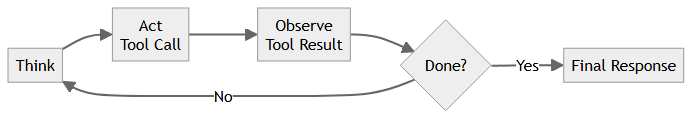
\includegraphics[width=0.75\textwidth]{images/react_cycle.png}
    \caption{ReAct Reasoning Cycle}
    \label{fig:react-cycle}
\end{figure}

\subsection{Multi-Provider Model Configuration}

\begin{table}[H]
    \centering
    \caption{Supported LLM Providers}
    \label{tab:llm-providers}
    \small
    \begin{tabular}{|l|l|l|}
        \hline
        \textbf{Provider} & \textbf{Interface} & \textbf{Use Case} \\
        \hline
        Ollama & Local HTTP API & Development, offline eval, privacy \\
        OpenAI & Chat Completions API & Production evaluation \\
        Self-hosted (fine-tuned) & OpenAI-compatible API & Domain-adapted local deployment \\
        \hline
    \end{tabular}
\end{table}

Configuration is per-session: main model (Observer/Operator reasoning), specialist model (planning/structured output), and temperature (0 for deterministic evaluation). The same system prompts are used across all providers to ensure behavioral differences reflect model capability.

\subsection{Instruction Design}

The \textbf{Observer} prompt defines tool categories, routing rules for Operator handoff, evidence requirements (responses must cite tool output), documentation retrieval triggers, and output structure.

The \textbf{Operator} prompt defines confirmation requirements for destructive operations, scope preservation rules, discovery-read permissions, error handling, and return protocol.

\subsection{Tool Calling Integration}

Two patterns are supported: (1)~native function calling (OpenAI) where structured JSON tool calls are validated and dispatched; (2)~text-based calling for models without native support, parsed by the runtime. Invalid parameters are rejected with feedback for self-correction.

Read-only tools may execute in parallel within a single reasoning step (e.g., \texttt{squeue}+\texttt{sinfo}+\texttt{sdiag} for cluster overview). Destructive tools always execute sequentially with confirmation.

\subsection{Context Management}

\begin{itemize}
    \item Chart artifacts stored separately, excluded from subsequent reasoning
    \item Large tool outputs truncated above a configurable threshold
    \item Session-scoped history with evaluation isolation per test case
\end{itemize}

\subsection{Streaming Events}

The structured stream carries: \texttt{token}, \texttt{thinking}, \texttt{tool\_start}, \texttt{tool\_result}, \texttt{chart\_artifact}, \texttt{pending\_action}, \texttt{todo\_update}, and \texttt{status} events. This provides real-time visibility for interactive use and structured trace data for evaluation scoring.

\subsection{Domain-Adapted Fine-Tuning}
\label{sec:fine-tuning}

While the system achieves strong results with commercial API models, reliance on external providers introduces latency, cost, and privacy concerns for production HPC environments. To address this, the project explores domain-adapted fine-tuning of an open-weight model as an alternative backbone for the agent.

\subsubsection{Distillation from Evaluation Traces}

The fine-tuning approach leverages a key insight: the evaluation framework already produces thousands of successful agent traces---complete records of how the commercial model correctly handled each benchmark case, including the exact sequence of tool calls, routing decisions, and final responses. These traces serve as high-quality training signal without requiring manual annotation.

The data construction pipeline processes each passing evaluation trace through several stages. First, the raw trace is parsed into a multi-turn conversation that follows the model's expected chat template format: a system prompt establishing the agent role, followed by alternating user messages, assistant reasoning with tool calls, and tool response observations. Each tool call is represented as a structured JSON object specifying the function name and arguments, matching the format that the model must learn to generate at inference time.

Second, the pipeline applies augmentation to increase diversity. Evaluation traces that involve an Observer-to-Operator handoff are split into two independent training samples at the handoff boundary. Traces are also augmented with minor prompt variations (rephrasing the user query) to reduce overfitting to specific evaluation phrasings.

The resulting dataset contains over 10{,}000 training samples---approximately 7{,}500 Observer conversations and 2{,}600 Operator conversations---stored in JSONL format where each line is a complete training example with three fields: the message history, the list of available tools for that role, and metadata for validation.

\subsubsection{Role-Scoped Tool Exposure}

A critical challenge discovered during initial fine-tuning was \emph{cross-role tool hallucination}: the model would call tools belonging to the wrong agent role---for example, an Observer-mode response invoking \texttt{scontrol\_hold} (a dangerous Operator tool) instead of delegating through the handoff mechanism.

The root cause was that the original training data presented all available tools as a single flat list regardless of which agent role was active. The model therefore never learned that tool availability is conditional on the current role context.

The solution is to split each training conversation at the handoff boundary, producing two independent samples with strictly scoped tool definitions:

\begin{itemize}
    \item The \textbf{Observer sample} includes only read-only and analysis tools plus the handoff mechanism, teaching the model that state-changing operations must be delegated rather than executed directly.
    \item The \textbf{Operator sample} includes only action tools and a subset of verification tools, teaching the model to execute within its granted scope and hand back when complete.
\end{itemize}

By embedding the tool boundary directly into the training data format, the model internalizes the Observer/Operator separation as part of its generation behavior rather than relying solely on runtime filtering.

% TODO: Add figure showing role-scoped training data split
% \begin{figure}[H]
%     \centering
%     \includegraphics[width=\textwidth]{images/role_scoped_training.png}
%     \caption{Role-Scoped Training Data Construction}
%     \label{fig:role-scoped-training}
% \end{figure}

\subsubsection{Training Configuration}

The fine-tuning uses parameter-efficient QLoRA adaptation, modifying only a small fraction of the base model's weights while preserving its general language capabilities. The procedure involves two aspects of preparation: quantizing the base model and configuring the low-rank adapter.

\paragraph{Model Preparation.}
The base model (Qwen2.5-14B-Instruct) is loaded in 4-bit NormalFloat (NF4) quantization with double quantization enabled, reducing the 14-billion parameter checkpoint from approximately 28\,GB to under 10\,GB in GPU memory. Computation is performed in bfloat16 precision for numerical stability. The model uses Grouped Query Attention (40 query heads sharing 8 key-value heads), which naturally benefits from the memory savings of quantization since the KV-cache overhead is already reduced by the GQA architecture.

A LoRA adapter with rank 64 and scaling factor $\alpha=128$ is attached exclusively to the final 12 transformer layers (layers 36--47 of 48 total). This targeting rationale is that lower layers encode general language representations already well-trained during pretraining, while the upper layers closest to the output are responsible for task-specific decision patterns---precisely what needs adaptation for tool-calling behavior. The adapter modifies the query, key, value, and output projection matrices in each targeted layer, adding roughly 180 million trainable parameters (about 1.3\% of the full model).

\paragraph{Data Formatting.}
Each training sample is rendered through the model's native chat template, which handles the conversion from the structured message list into the token sequence the model expects. Critically, the per-sample \texttt{tools} field is passed directly to the template engine, so the model sees the tool definitions as part of its input context---exactly as it would at inference time. The template marks assistant tool-call outputs with special tokens that the loss function targets, while masking system prompts and user messages from the gradient computation. This ensures the model is trained only to generate the correct assistant responses and tool invocations, not to memorize the prompts.

\paragraph{Training Procedure.}
Training runs for 3 epochs with an effective batch size of 16 (micro-batch 4 $\times$ gradient accumulation 4), maximum sequence length of 2{,}048 tokens, and the AdamW optimizer with a cosine learning rate schedule. Gradient checkpointing with non-reentrant mode is enabled to trade computation for memory, allowing the full procedure to fit within a single 48\,GB A40 GPU. Sequences exceeding the length limit are truncated from the right, which primarily affects long multi-tool traces where the final response is cut---an acceptable trade-off since the tool-calling patterns in the earlier turns are preserved.

% TODO: Add figure showing training loss curve from wandb
% \begin{figure}[H]
%     \centering
%     \includegraphics[width=0.8\textwidth]{images/training_loss_curve.png}
%     \caption{Fine-Tuning Loss Curve}
%     \label{fig:training-loss}
% \end{figure}
